% !TEX root = ../main.tex
\section{Introduction}    

\begin{frame}{Introduction} 

    \begin{block}{Keyword Spotting definition}
        \textbf{Keyword Spotting} - process of identifying pre-defined keywords, in speech recorded in real-time.
    \end{block}

    \begin{columns}
        \begin{column}{0.4\textwidth}
            \begin{block}{Keyword Spotting in real world}
                \textbf{Wakeup Word} - common way to begin an interaction by the voice interface.
            \end{block}
            \begin{exampleblock}{Example}
                \begin{itemize}
                    \item Amazon - ``Alexa''
                    \item Google - ``OK Google''
                    \item Apple - ``Hey Siri''
                \end{itemize}
            \end{exampleblock}
        \end{column}

        \begin{column}{0.6\textwidth}            
            \begin{figure}
                \centering
                \begin{subfigure}[b]{0.49\textwidth}
                    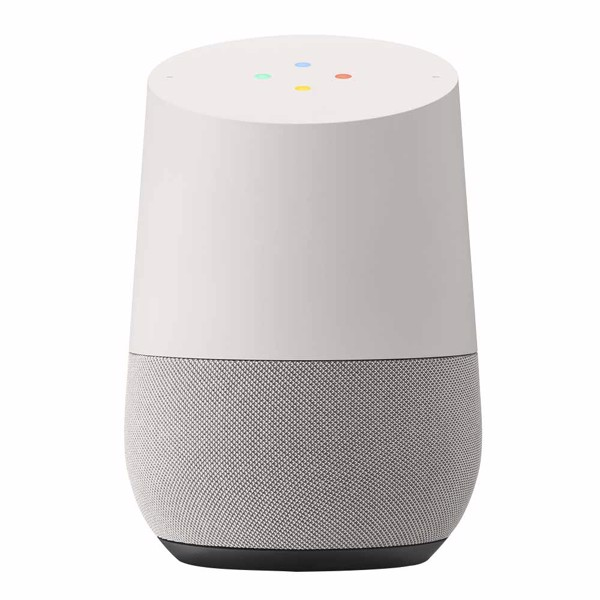
\includegraphics[width=\textwidth]{figure/google_home.png}
                \end{subfigure}
                \centering
                \begin{subfigure}[b]{0.49\textwidth}
                    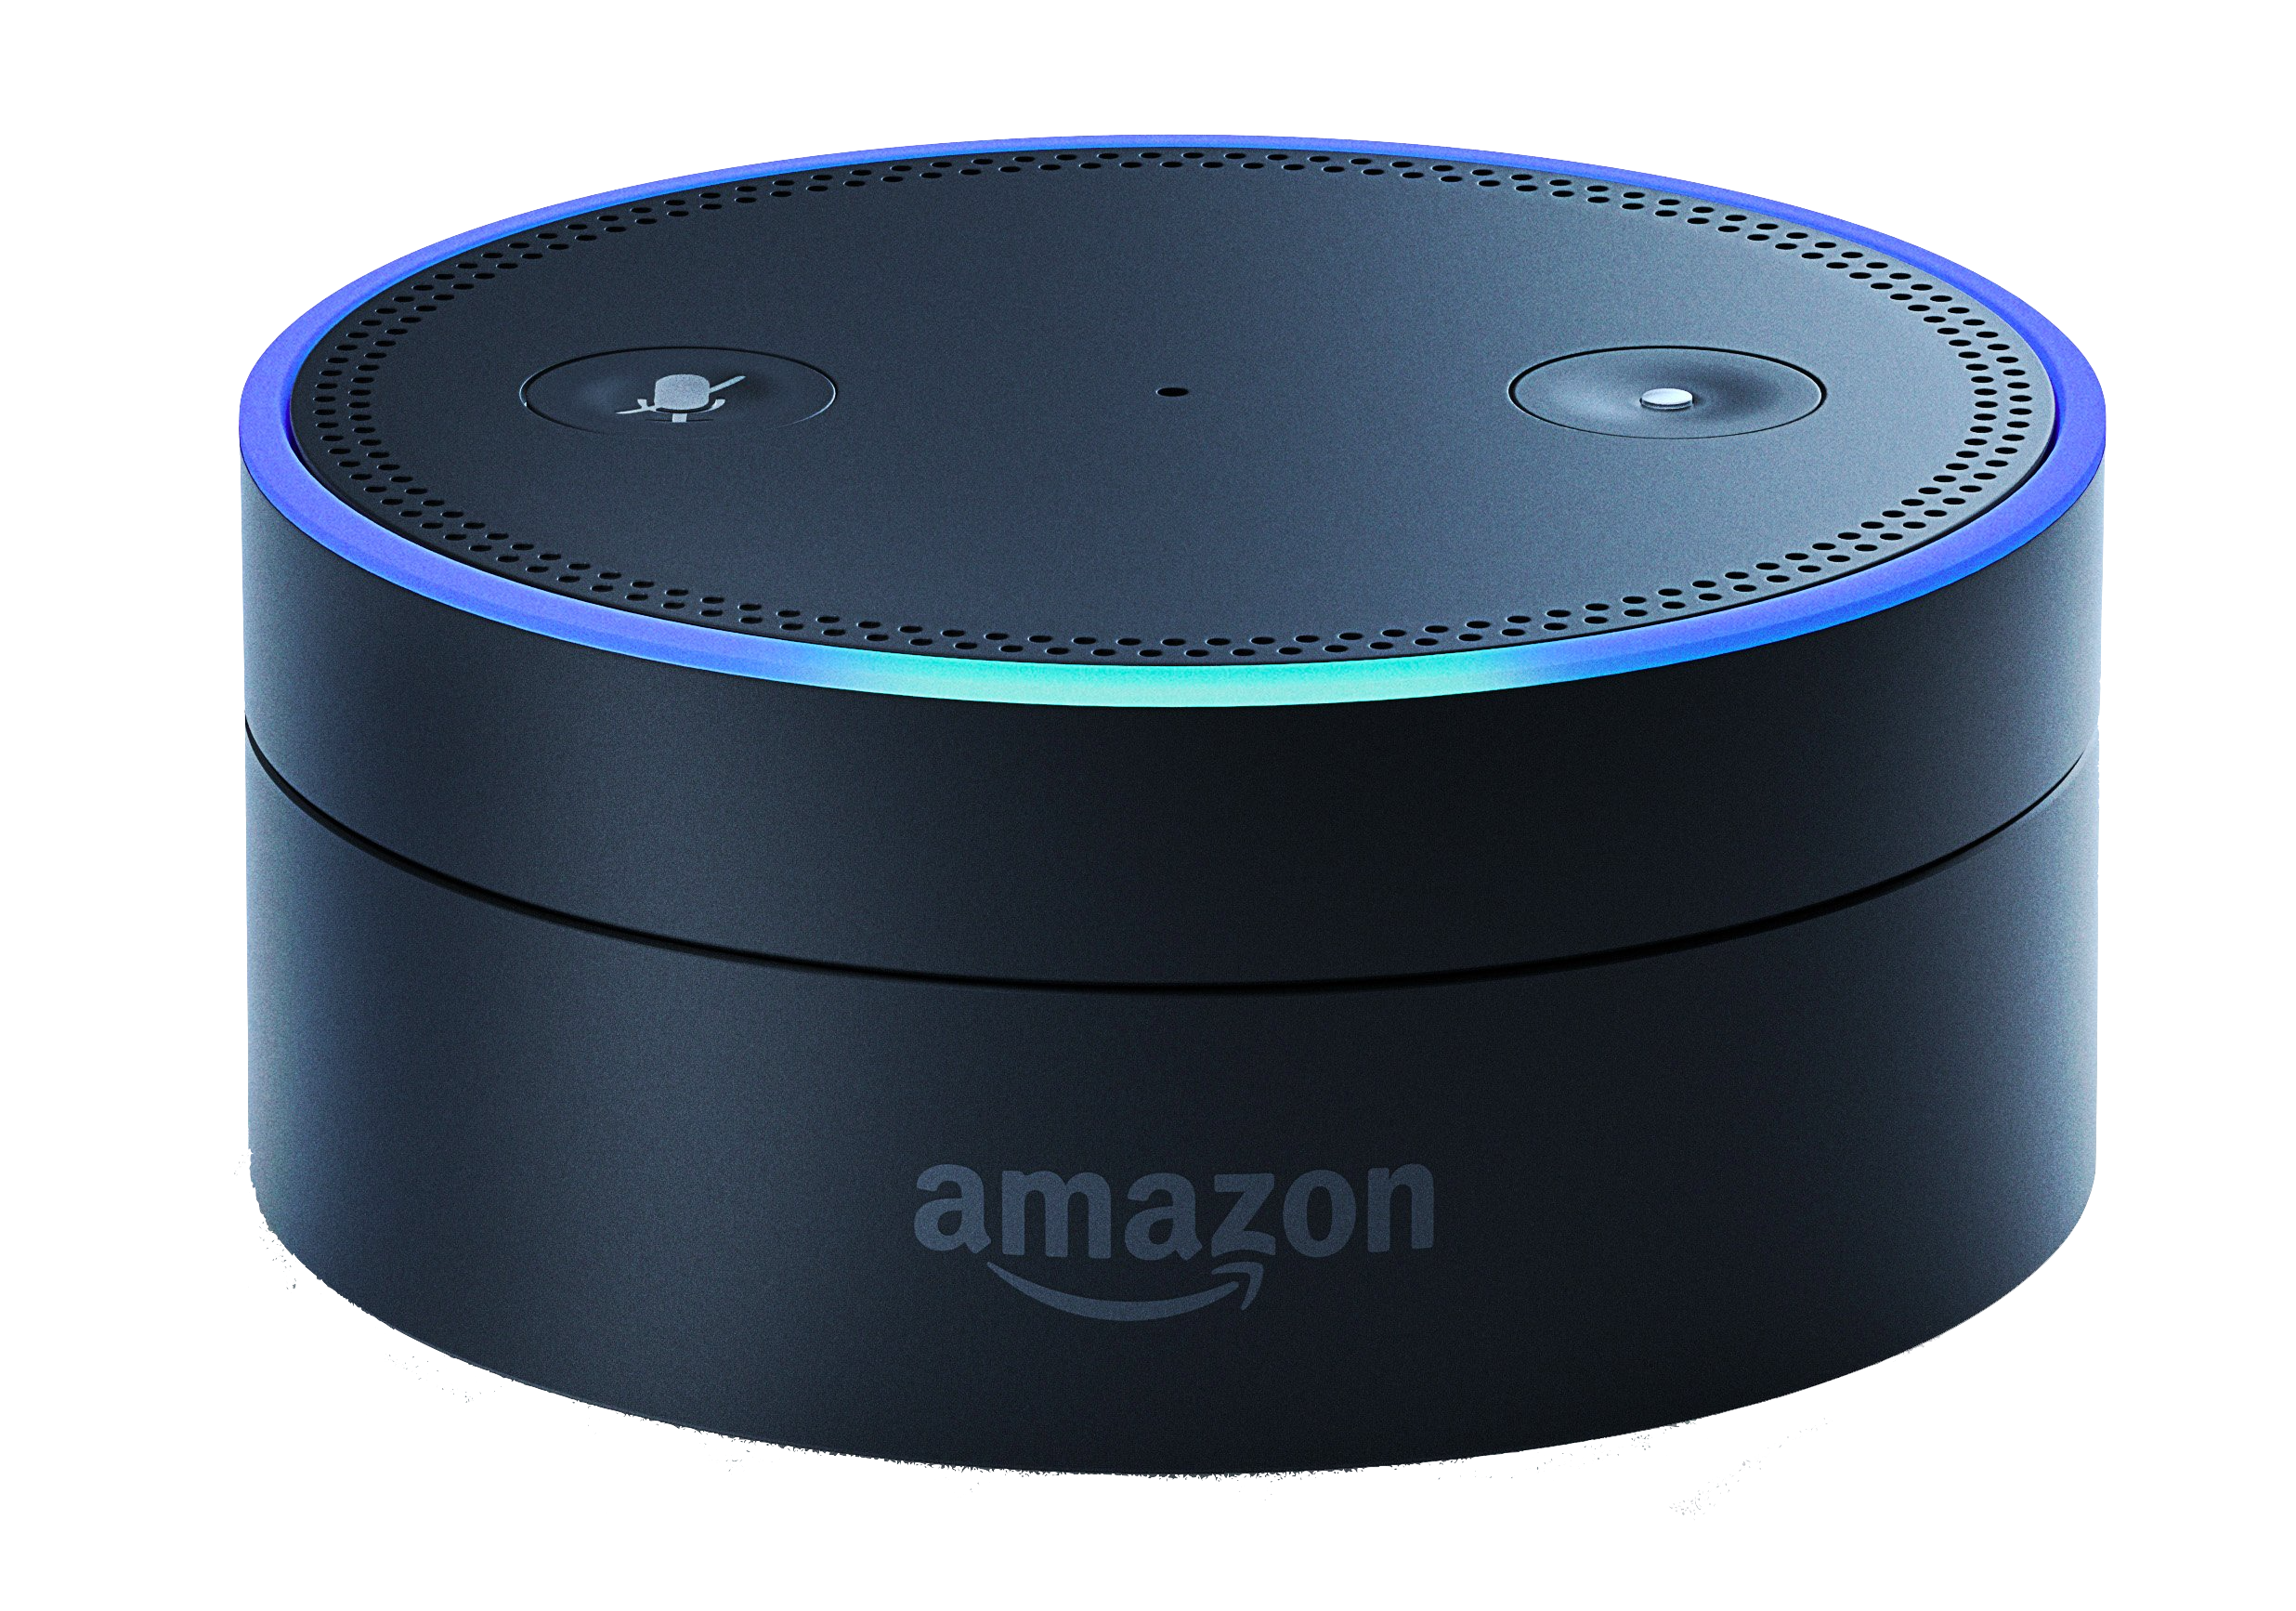
\includegraphics[width=0.8\textwidth]{figure/amazon_echo.png}
                \end{subfigure}
                \caption{Keyword spotting on production.}
            \end{figure}    
        \end{column}
    \end{columns}
\end{frame}

